\chapter{Referencial Teórico}

Neste capítulo será explorado o referencial teórico que servirá de suporte teórico e contextual para o desenvolvimento desta pesquisa. Para tanto, realizou-se uma detalhada revisão de literatura, contemplando os principais conceitos relacionados ao tema de estudo. 

\section{Saúde e Bem-estar}

O conceito de saúde é um dos mais complexos e discutidos no campo da medicina. Embora a primeiro momento pareça um termo simples e autoexplicativo, várias versões são apresentadas em sua definição. Segundo \citeonline{moacyr_scliar_2007}, o termo não possui um único significado, mas reflete a conjuntura social, econômica, política e cultural de cada um, e depende do lugar, da época e da classe social além de valores individuais e de concepções científicas, religiosas e filosóficas.

Para \citeonline{christopher_boorse}, por exemplo, o termo se resumia apenas à ausência de doença. Essa ideia chocava-se com o que era difundido pela Organização Mundial da Saúde (OMS) à partir da divulgação da carta de princípios de 7 de abril de 1948 que dizia que “Saúde é o estado do mais completo bem-estar físico, mental e social e não apenas a ausência de enfermidade" \cite{moacyr_scliar_2007}. É essa concepção ampliada que valoriza múltiplas fatores do bem-estar que servirá como base para o desenvolvimento deste projeto.

Afinal, entender o termo "saúde" apenas como a ausência de enfermidades é reduzir a complexidade da experiência humana e ignorar variáveis cruciais que afetam diretamente a qualidade de vida dos indivíduos. Sob esse prisma surgiu o Relatório de Lalonde (1974), que determinava que a saúde poderia ser classificada em quatro áreas gerais, sendo elas: biologia, ambiente, estilo de vida e organização dos serviços de saúde \cite{lalonde}. Essas seriam consideradas determinantes da saúde pelo autor, que destacou ainda os impactos dos hábitos de vida individuais na própria saúde \cite{lalonde}.

Com base nessa perspectiva e com a pretensão de iniciar um monitoramento de saúde de indivíduos, propõe-se, neste trabalho, resumir as seções de biologia e de organização dos serviços de saúde em questões de disposições genéticas e de avaliação de acesso a saúde. Assim, os tópicos referentes ao estilo de vida e ao ambiente ganham maior extensibilidade e contemplam questões como hábitos alimentares, prática de exercícios físicos, uso de substâncias, frequência de interações sociais, condições de moradia, entre outros.

Vale ressaltar que a síntese de dois tópicos tão importantes enquanto determinantes da saúde não implica necessariamente em uma diferença de complexidade entre as variáveis. Essa opção reflete apenas uma decisão metodológica do projeto que busca concentrar esforços analíticos em aspectos sobre os quais, acredita-se que uma instituição de ensino superior teria maior autonomia para promover mudanças significativas. Dessa forma optou-se pela simplificação do levantamento de dados relativos à biologia e à organização de serviços de saúde, em razão de serem variáveis mais distantes da esfera de atuação dessas instituições de ensino.

\subsection{Estilo de Vida e Ambiente}

Nestas duas categorias de determinantes da saúde citadas por \citeonline{lalonde}, alguns estudos mostram que existe uma forte correlação entre ambas. Os resultados obtidos por \citeonline{muniz2021mudanccas}, por exemplo, de forma análoga a outros estudos mencionados no artigo, concluem que o meio universitário impacta diretamente na saúde física e mental dos estudantes ao impor exigências que levam a sobrecarga dos estudantes. Esta é mais uma razão que reforça a necessidade de monitoramento de hábitos no cenário universitário e a implementação de estratégias para contornar hábitos ruins dentro dessas instituições.

Além de avaliação de ambiente acadêmico seria interessante também contemplar dados à respeito do ambiente de trabalho e familiar, uma vez que esses fatores exercem grande impacto na saúde mental e do bem-estar dos indivíduos.

No que diz respeito a um estilo de vida que promova a saúde e o bem-estar, além da óbvia necessidade biológica vital de hidratação do próprio organismo, incluem-se práticas de atividades físicas, alimentação equilibrada, regularidade no ciclo do sono \cite{arlinghaus2019importance}, interações sociais, voluntariado \cite{helliwell2025world} e momentos de lazer \cite{batista2012lazer}. 

Dessa forma seções de avaliação destes aspectos na vida cotidiana serão implementadas no aplicativo para acompanhamento da saúde geral da comunidade universitária.

\subsection{Saúde Mental}

Como vimos, a saúde não se resume fatores biológicos favoráveis. Aqui é posto a saúde mental em uma seção exclusiva para se avaliar já que ela envolve parâmetros profundamente subjetivos e complexos que ultrapassam o cumprimento de rotinas que visam o bem-estar, embora a existência de fortes correlações entre a prática de bons hábitos e melhoria do estado emocional. Contudo, essas correlações não esclarecem todas as condições clínicas geradas por doenças mentais \cite{quartilho2010saude}.

Comenta-se em uma separação do cérebro e da mente que não nos possibilita tratar questões de saúde mental com uma explicação linear de experiências conscientes \cite{quartilho2010saude}. Dessa forma, mesmo com um bom estilo de vida, é possível que ainda aja uma saúde mental comprometida.

Esta variável é crucial de ser analisada, principalmente quando vimos que antes mesmo de um período pandêmico - e, por mais que não seja uma atribuição direta da Universidade de sanar este problema - já se tratava de uma das maiores reinvindicações entre os alunos da Universidade de Brasília, sendo uma das principais razões de evasão acadêmica \cite{oliveira2020acesso}. Com os agravantes do contexto pós-pandemia essa questão se tornou ainda mais importante de ser avaliada \cite{da2025saude}.

% determinantes

%\section{Promoção da Saúde}

%- citar DASU

%- citar ferramentas/serviços unb

%- proj extensão

\section{Plataformas Existentes}

Para a execução deste trabalho, foi previamente realizado um levantamento de dados sobre aplicativos com propostas semelhantes de monitoramento de hábitos e do estado de saúde mental. 

O Habitica, mostrado na Figura~\ref{habitica}, foi um dos softwares encontrados neste levantamento. O aplicativo de código aberto tem como funcionalidade principal amparar a formação de hábitos novos por meio da gamificação. Ele funciona como uma combinação de rede social e um jogo pois a ferramenta te permite adicionar amigos e combater monstros em missões com eles conforme você realiza suas tarefas diárias. Cada tarefa concluída na vida real, quando registrada no aplicativo, concede pontos de experiência ao usuário que se engaja na realização de suas próprias tarefas para evoluir no jogo \cite{habitica}. 


\begin{figure}[H]
    \centering
    \caption{Tela inicial do Habitica}
    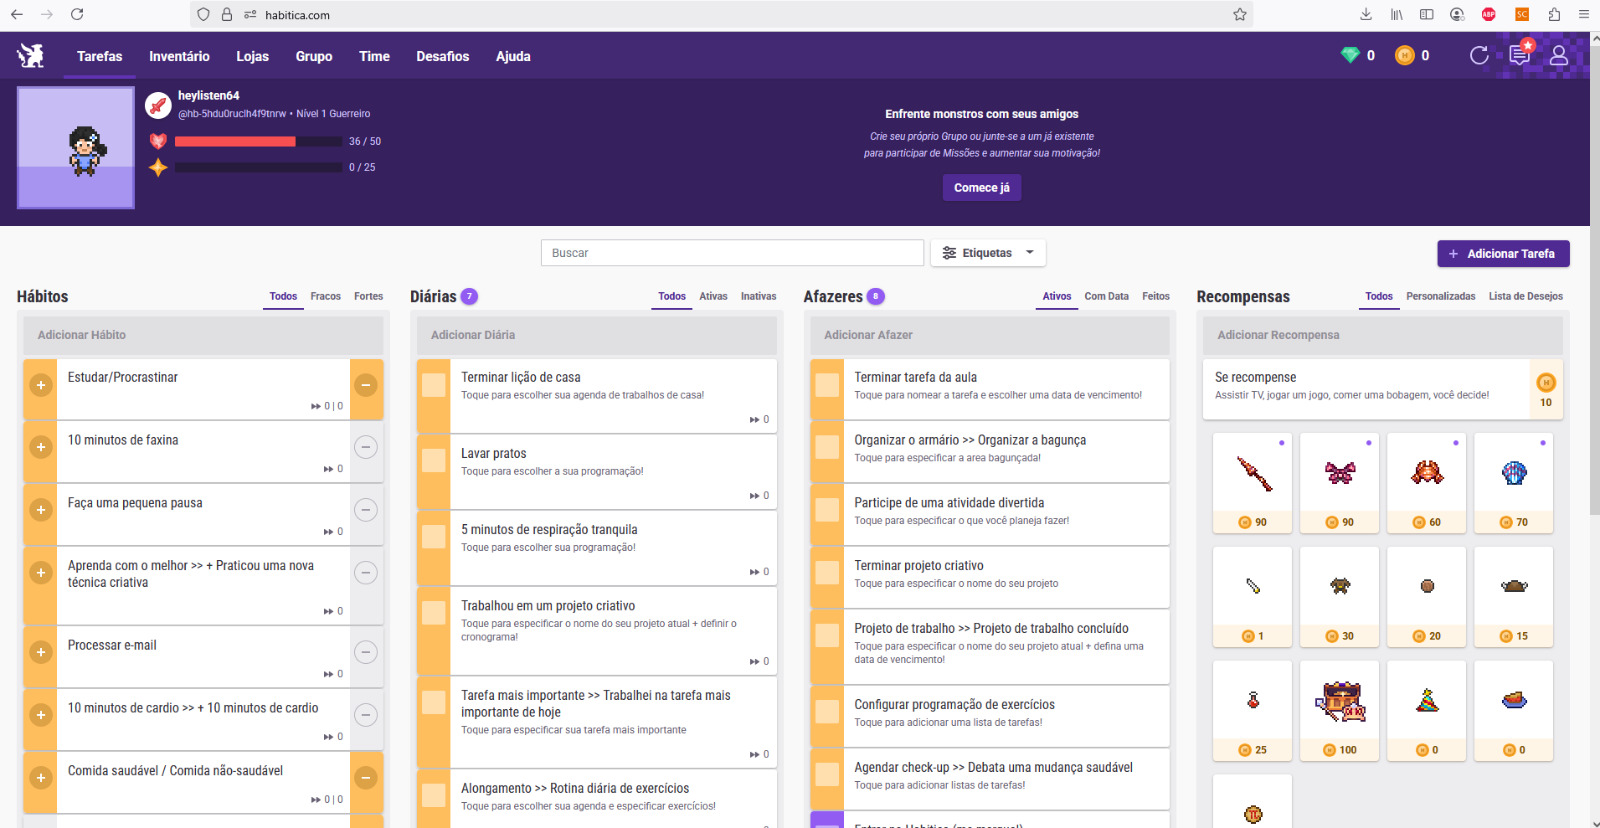
\includegraphics[width=1\linewidth]{figuras/habitica.jpg}
    \par
    Fonte: \cite{habitica}.
    \par
    \label{habitica}
\end{figure}

Porém, em comparação a este sistema, o projeto em desenvolvimento se destaca por oferecer conteúdos de direcionamento personalizados dispostos em um feed dinâmico que se adapta de acordo com a progressão individual do usuário nas diversas seções do bem-estar dispostas no projeto. Dicas, eventos específicos e demais informações relacionadas aos temas em que o usuário apresenta um progresso insatisfatório são exibidos para ele nesse espaço.

Já o Daylio se intitula como um diário de autocuidado que registra diariamente o humor e rastreia a felicidade do usuário sem a necessidade de escrita, registrando hábitos apenas com emojis, o que torna a usabilidade mais amigável \cite{daylio}. Nele registramos nosso humor e a partir daí selecionamos outras opções que permeiam o nosso estado emocional, como qualidade do sono, interações sociais, frequência em atividades físicas, entre outros. Assim, o aplicativo traça, de registros simples de humor a estatísticas de correlação entre essas diferentes variáveis.

\begin{figure}[H]
    \centering
    \caption{Telas do Daylio}
    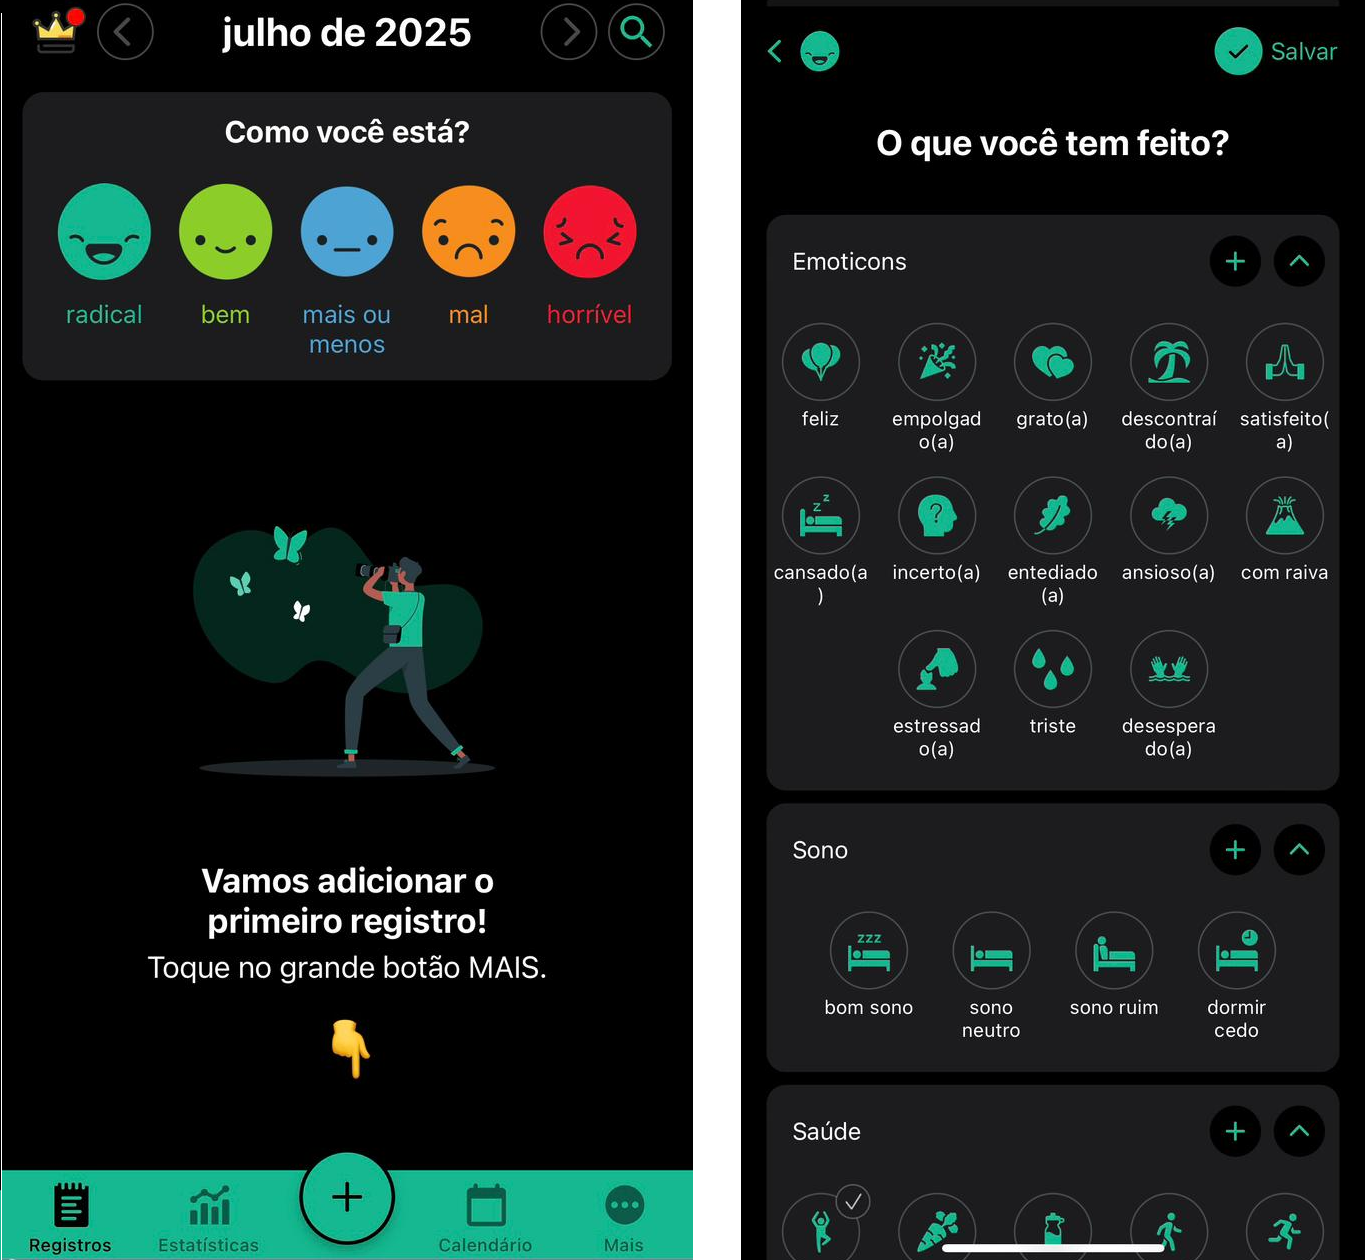
\includegraphics[width=0.75\linewidth]{figuras/telasdaylio.png}
    \par
    Fonte: \cite{daylio}.
    \par
    \label{daylio}
\end{figure}

Entretanto nenhum dos softwares encontrados mostraram-se como uma ferramenta conjunta entre uma instituição específica e seus respectivos membros. A solução deste trabalho consiste em uma ferramenta que forneça dados da comunidade universitária e beneficie não apenas o usuário - que passa a tomar consciência de seus comportamentos por feedbacks de progressos - como também a própria instituição que poderá acompanhar indicadores coletivos e planejar ações direcionadas de promoção da saúde e consequentemente ter membros mais saudáveis e engajados em seu ambiente.

As plataformas também não oferecem uma seleção básica de seções de bem-estar, variáveis que este trabalho propõe monitorar de forma estruturada.

% \section{Heurísticas de Nielsen}

% Segundo \citeonline{nielsen_1994} existem dez princípios amplamente conhecido para proporcionar usabilidade a um sistema, conhecido como Dez Heurísticas de Nielsen. Esses princípios funcionam como diretrizes para o desenvolvimento de interfaces mais intuitivas, eficientes e centradas no usuário, sendo essas diretrizes:

% \begin{enumerate}
%     \item \textbf{Visibilidade do status do sistema}: O sistema deve sempre manter os usuários informados sobre o que está acontecendo, por meio de feedback apropriado em tempo razoável.
    
%     \item \textbf{Correspondência entre o sistema e o mundo real}: A interface deve falar a linguagem do usuário, com palavras, frases e conceitos familiares, seguindo convenções do mundo real.
    
%     \item \textbf{Controle e liberdade do usuário}: Usuários frequentemente escolhem funções por engano; é necessário oferecer mecanismos claros de desfazer e refazer ações.
    
%     \item \textbf{Consistência e padrões}: Os usuários não devem ter que imaginar se diferentes palavras, situações ou ações significam a mesma coisa. O sistema deve seguir convenções.
    
%     \item \textbf{Prevenção de erros}: Melhor do que apresentar boas mensagens de erro é evitar que o erro ocorra, por meio de design cuidadoso.
    
%     \item \textbf{Reconhecimento em vez de memorização}: Minimizar a carga de memória do usuário, tornando objetos, ações e opções visíveis.
    
%     \item \textbf{Flexibilidade e eficiência de uso}: A interface deve atender tanto usuários iniciantes quanto experientes, permitindo atalhos para os mais avançados.
    
%     \item \textbf{Estética e design minimalista}: Diálogos e telas não devem conter informações irrelevantes ou raramente necessárias.
    
%     \item \textbf{Ajuda no reconhecimento, diagnóstico e recuperação de erros}: As mensagens de erro devem ser expressas em linguagem simples, indicando claramente o problema e sugerindo uma solução.
    
%     \item \textbf{Ajuda e documentação}: Mesmo que o sistema possa ser utilizado sem documentação, pode ser necessário oferecer ajuda e instruções acessíveis e objetivas.
% \end{enumerate}

% Sendo assim, a fim de proporcionar usabilidade e acessibilidade a todos os publicos o projeto proposto visa a utilização das heuristicas, como também visa seguir as normas da LGPD (Lei Geral de Proteção) a fim de proporcionar maior segurança aos usuários \cite{brasil2018lgpd}.

% \section{Escala de Likert}

% A Escala de Likert é uma das principais ferramentas psicométricas, sendo amplamente utilizada nas pesquisas em ciências sociais e educacionais. Ela foi desenvolvida com o principal objetivo de quantificar atitudes, percepções e crenças, sendo uma maneira de transformar fenômenos qualitativos da experiência humana em dados quantificáveis e cientificamente tratáveis \cite{joshi_2015}.

% Além disso, do ponto de vista psicométrico, a Escala de Likert proporciona a mensuração de variáveis latentes, como sentimento ou opiniões, por meio de afirmações com os quais os participantes expressam níveis de concordância ou discordância em uma escala ordinal simétrica. Em outras palavras, a escala apresenta cinco ou sete pontos, indo de "discordo totalmente" até "concordo totalmente", permitindo capturar nuances mais refinados, sendo preferível a escala com sete pontos, pois proporciona mais opções intermediárias ao participante, o que aumenta a precisão da medida psicométrica \cite{joshi_2015}.

% Sendo assim, a Escala de Likert é fundamental para a avaliação de atitudes e percepções de natureza psicológica, proporcionando uma coleta de dados mais precisa, coerente e passível de análise estatística. Portanto, é uma ferramenta indispensável para a realização de formulários sobre o bem-estar e hábitos.

% \section{Alpha de Cronbach}

% O Alpha de Cronbach, proposto por Lee Cronbach em 1951, é uma maneira de avaliar quão fidedigno é um conjunto de dados. Em outras palavras, ele verifica o quanto as perguntas estão correlacionadas entre si, o que permite avaliar a confiabilidade dos dados \cite{cronbach_1951}. Sendo assim, é possível calcula-lo a partir da seguinte equação:

% \begin{equation}
% \label{eqn01}
%     \mathbf{\alpha} = \frac{N}{N - 1} \left( 1 - \frac{\sum_{i=1}^{N} \sigma_{Y_i}^2}{\sigma_X^2} \right)
% \end{equation}

% % Onde:

% % \begin{itemize}
% % \item[$ \alpha $] Coeficiente de confiabilidade (Alpha de Cronbach)
% % \item[$ N $] Número total de itens no conjunto de perguntas
% % \item[$ \sigma_{Y_i}^2 $] Variância do i-ésimo item
% % \item[$ \sigma_X^2 $] Variância total do somatório dos itens
% % \item[$ \sum $] Somatório dos itens
% % \end{itemize}

% Além de indicar a confiabilidade dos dados coletados, o Alpha de Cronbach também permite verificar a concordância entre as perguntas. Isso é útil para avaliar se o conjunto de questões está bem estruturado e se mede de forma coerente o mesmo conceito \cite{cronbach_1951}.

% O cálculo do Alpha de Cronbach pode ser implementado em qualquer linguagem de programação Turing-completa, como Java, python, entre outras linguagens de programação modernas. Ou seja, a equação independe da linguagem de programação, sendo versátil e adaptável.

% Em suma, o valor do Alpha de Cronbach varia entre -1 e 1, sendo que valores próximos de 1 ou -1 indicam alta confiabilidade. Sendo assim, basta introduzir o conjunto de dados ao algoritmo que implementa a equação do Cronbach e considera-se que valores acima de 0.6 ou menores que -0.6 possuem dados confiáveis. Contudo, valores muito baixos ou negativos indicam pouca ou nenhuma confiabilidade \cite{cronbach_1951}.

